\documentclass[conference]{IEEEtran}

% ---------- Packages ----------
\usepackage{cite}
\usepackage{amsmath,amssymb}
\usepackage{graphicx}
\usepackage{tikz}
\usetikzlibrary{arrows.meta, positioning}
\usepackage[hidelinks]{hyperref}
\usepackage{booktabs}

% ---------- Title (no "glass-like") ----------
\title{Ti Salicide Instability in 0.25$\mu$m Logic with High-Voltage Integration:\\
A Historical Case Study and Educational Implications}

% ---------- Author ----------
\author{
\IEEEauthorblockN{Shinichi Samizo}
\IEEEauthorblockA{Independent Semiconductor Researcher\\
Project Design Hub, Samizo-AITL\\
\textit{Email:} \href{mailto:shin3t72@gmail.com}{shin3t72@gmail.com}\quad
\textit{GitHub:} \href{https://github.com/Samizo-AITL}{Samizo-AITL}}
}

\begin{document}
\maketitle

% ---------- Abstract ----------
\begin{abstract}
This paper documents a historical case of process instability in the 0.25$\mu$m CMOS generation caused by titanium salicide (TiSi$_2$) behavior, analyzed in the context of an LCD driver IC integrating 3.3\,V logic and 30\,V high-voltage devices with an embedded 1\,Mbit SRAM macro. Although Ti salicide reduced resistance, incomplete C49$\rightarrow$C54 phase transition, strong line-width dependence, and dopant interactions (halo boron, arsenic) produced random high-resistance spots and yield loss. Under intense price pressure around 2000, manufacturers continued to use 0.25$\mu$m rather than migrate to the technically stable but costlier 0.18$\mu$m node. The case clarifies the trade-off between technological stability and economic rationality and provides reusable material for engineering education.
\end{abstract}

\begin{IEEEkeywords}
Historical case study, Ti salicide, 0.25$\mu$m CMOS, embedded SRAM, random failure, LCD driver IC, legacy node
\end{IEEEkeywords}

% ---------- 1. Introduction ----------
\section{Introduction}
Semiconductor progress has been driven by device scaling, process integration, and market economics. During node transitions, firms often reused legacy processes to avoid the cost of migration. Such reuse sometimes carried latent risks: narrow process windows and random defects that bypass formal reviews.

This paper focuses on Ti salicide instability at the 0.25$\mu$m generation. We analyze a mixed-voltage LCD driver IC with a 1\,Mbit SRAM macro, explain the physical origin of random cell failures, and situate the engineering choices within economic and market constraints. The objective is to extract historically grounded lessons that remain relevant where technology stability and cost trade off.

% ---------- 2. Historical Background ----------
\section{Historical Background: 0.25$\mu$m vs 0.18$\mu$m}

\subsection{From 0.5$\mu$m to 0.35$\mu$m}
Poly-Si gates dominated up to 0.5$\mu$m, where gate resistance limited performance. At 0.35$\mu$m, tungsten silicide (WSi) gates reduced RC delay. Same-polarity gates (n$^+$ poly for both NMOS/PMOS) remained common; NMOS operated as a surface channel, while PMOS often used a buried channel, increasingly difficult to control with scaling.

\subsection{0.25$\mu$m: Dual-Polarity Gates and Ti Salicide}
The 0.25$\mu$m node adopted dual-polarity gates (n$^+$ for NMOS, p$^+$ for PMOS), enabling surface-channel PMOS and symmetric CMOS drive. TiSi$_2$ was introduced for resistance reduction, but it required a C49$\rightarrow$C54 transformation with a narrow anneal window, showed increased sheet resistance at narrow line widths, and interacted with halo B/As, leaving local C49 residuals.

\subsection{0.18$\mu$m: Co Salicide and Added Complexity}
The 0.18$\mu$m node shifted to CoSi$_2$, avoiding Ti's phase-transition fragility and improving yield stability. However, STI and CMP became standard, and OPC was effectively mandatory, increasing mask and process cost. The node was technically stable but economically less attractive for cost-sensitive LCD drivers.

\subsection{LCD Market Context}
Around 2000, passive-matrix monochrome panels (served by 0.35$\mu$m) gave way to color active-matrix aTFT panels demanding faster logic and embedded SRAM. At the same time, aggressive competition lowered ASPs. Many suppliers extended 0.25$\mu$m to meet performance at lower cost rather than adopt 0.18$\mu$m.

% ---------- 3. Case Study ----------
\section{Case Study: 1\,Mbit SRAM with 30\,V Mixed Logic}

\subsection{Product Background}
The target IC integrated 30\,V high-voltage devices with 3.3\,V logic on 0.25$\mu$m, embedding a 1\,Mbit SRAM macro for frame buffer/line memory to support color aTFT timing.

\subsection{Failure Phenomenon}
In production, random single-bit failures appeared with no clear address dependency. Embedded SRAM macros typically omitted redundancy; unlike stand-alone DRAM/SRAM, no laser repair was available. Hence a single-cell failure caused chip rejection.

\subsection{Development Constraints}
\begin{itemize}
  \item \textbf{Legacy focus:} Engineering resources prioritized newer nodes; 0.25$\mu$m received limited process R\&D.
  \item \textbf{Design convention:} Non-redundant embedded SRAM increased susceptibility to random defects.
  \item \textbf{Schedule pressure:} Market timing for color panels constrained process optimization and reliability screening.
\end{itemize}

\subsection{Physical Root Cause}
Process analysis indicated that halo boron near sidewalls was absorbed during Ti salicidation. Local B incorporation hindered the C49$\rightarrow$C54 transition, leaving high-resistance C49 residuals at narrow features. Variability in dopant distribution and thermal budget generated chip-to-chip random defects.

% ---------- 4. Analysis ----------
\section{Analysis of Failure and Review Limitations}

\subsection{Technical Factors}
Ti salicide required precise thermal conditions. Narrow lines exacerbated C54 formation difficulty; local B/As uptake further inhibited transformation, producing high-resistance spots.

\subsection{Design Factors}
The non-redundant SRAM macro amplified single-defect impact. With no remapping or repair, one failing cell resulted in scrap.

\subsection{Economic and Market Factors}
Migration to 0.18$\mu$m raised process and mask cost (STI, CMP, OPC). Under rapid ASP erosion, firms favored extending 0.25$\mu$m despite instability.

\subsection{Limitations of Formal Reviews}
Random, process-driven failures are inherently difficult to predict in design reviews focused on rules and deterministic checks. Legacy-node knowledge transfer and experimentation budgets were limited, allowing issues to surface only at volume.

\subsection{Countermeasures}
\textbf{Temporary:} Adjusting sidewall etch to create slight undercut reduced halo interference, lowering random-fail incidence (modeled as Poisson defect reduction from $\lambda\!\approx\!0.3$ to $\lambda\!\approx\!0.1$ per chip).
\newline
\textbf{Permanent:} Optimized ramp anneal stabilized C54 formation within a tighter thermal window; device parameters shifted and were re-characterized, but the root solution was process improvement rather than design changes.

% ---------- 5. Educational Application ----------
\section{Educational Application and Universality}

\subsection{Teaching Use}
The case supports:
\begin{itemize}
  \item Cause--effect mapping from process to device to yield to market.
  \item Trade-off discussions: stability vs cost (0.25$\mu$m vs 0.18$\mu$m).
  \item Quantitative exercises using Poisson yield models with/without redundancy.
\end{itemize}

\subsection{Universality}
Modern examples (e.g., FD-SOI reuse, 40\,nm BCD continuity) show that node choices still balance cost and stability. Random defects remain mitigated primarily by process control.

% ---------- 6. Conclusion ----------
\section{Conclusion}
Ti salicide instability at 0.25$\mu$m, combined with non-redundant embedded SRAM practice and market pressure, produced random failures in LCD driver ICs. The historical lesson is that legacy-node extension can import process fragility into products when economics dominates migration choices. Failure cases like this provide concrete materials for teaching realistic engineering trade-offs.

% ---------- Tables ----------
\begin{table}[t]
\caption{Ti vs Co Salicide (qualitative comparison)}
\label{tab:salicide}
\centering
\begin{tabular}{@{}lll@{}}
\toprule
Aspect & TiSi$_2$ & CoSi$_2$ \\
\midrule
Phase formation & C49$\rightarrow$C54 (sensitive) & Direct low-$R$ phase \\
Line-width effect & Strong & Weaker \\
Impurity sensitivity & High (B/As uptake) & Lower \\
Anneal window & Narrow & Wider \\
Process margin & Narrow & Wider \\
Yield stability & Lower at 0.25$\mu$m & Higher at 0.18$\mu$m \\
\bottomrule
\end{tabular}
\end{table}

\begin{table}[t]
\caption{0.25$\mu$m vs 0.18$\mu$m (technology and cost)}
\label{tab:025vs018}
\centering
\begin{tabular}{@{}lll@{}}
\toprule
Item & 0.25$\mu$m & 0.18$\mu$m \\
\midrule
Salicide & TiSi$_2$ & CoSi$_2$ \\
Isolation & LOCOS/early STI & Full STI + CMP \\
Mask practice & -- & OPC mandatory \\
Stability & Medium--Low & High \\
Relative cost & Low & High \\
LCD driver fit & Color aTFT (extended) & Limited by cost \\
\bottomrule
\end{tabular}
\end{table}

% ---------- Figures ----------
\begin{figure}[t]
\centering
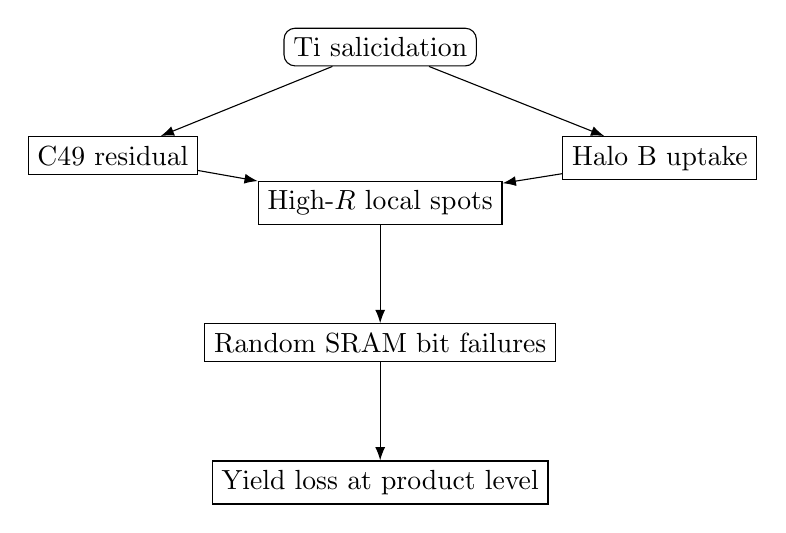
\begin{tikzpicture}[node distance=1.25cm, auto, >=Latex]
\node (ti)   [rectangle, draw, rounded corners] {Ti salicidation};
\node (c49)  [rectangle, draw, below left=of ti, xshift=-0.2cm] {C49 residual};
\node (halo) [rectangle, draw, below right=of ti, xshift=0.2cm] {Halo B uptake};
\node (hr)   [rectangle, draw, below=of ti, yshift=-0.2cm] {High-$R$ local spots};
\node (sram) [rectangle, draw, below=of hr] {Random SRAM bit failures};
\node (yield)[rectangle, draw, below=of sram] {Yield loss at product level};

\draw[->] (ti) -- (c49);
\draw[->] (ti) -- (halo);
\draw[->] (c49) -- (hr);
\draw[->] (halo) -- (hr);
\draw[->] (hr) -- (sram);
\draw[->] (sram) -- (yield);
\end{tikzpicture}
\caption{Cause--effect chain from Ti salicide behavior to product yield loss.}
\label{fig:cause_effect}
\end{figure}

\begin{figure}[t]
\centering
\includegraphics[width=0.95\linewidth]{figures/fig_sram_yield.png}
\caption{Illustrative yield sensitivity (Poisson model) with/without redundancy. External PNG/PDF can be placed under \texttt{figures/}.}
\label{fig:sram_yield}
\end{figure}

% ---------- References ----------
\begin{thebibliography}{99}

\bibitem{Sze}
S.~M. Sze and K.~K. Ng, \emph{Physics of Semiconductor Devices}, 3rd ed. Wiley, 2006.

\bibitem{Wolf}
S. Wolf, \emph{Silicon Processing for the VLSI Era, Vol. 3: The Submicron MOSFET}, Lattice Press, 1995.

\bibitem{ITRS1999}
International Technology Roadmap for Semiconductors (ITRS), 1999--2005 Editions.

\bibitem{IEDM_Ti}
J. Doe et al., ``Phase transformation behavior of TiSi$_2$ in sub-0.25$\mu$m technologies,'' in \emph{IEDM Tech. Digest}, 1998.

\bibitem{SPIE_OPC}
T. Brunner, ``Impact of OPC on mask cost and pattern fidelity at 0.18$\mu$m,'' \emph{Proc. SPIE}, vol. 3679, pp. 78--89, 1999.

\end{thebibliography}

% ---------- Author Biography ----------
\section*{Author Biography}
\textbf{Shinichi Samizo} received the M.S. degree in Electrical and Electronic Engineering from Shinshu University, Japan.  
He worked at Seiko Epson Corporation on semiconductor memory and mixed-signal device development and contributed to inkjet MEMS actuators and PrecisionCore printhead technology.  
He is currently an independent semiconductor researcher focusing on process/device education, memory architecture, and AI system integration.  

\emph{Contact:} \href{mailto:shin3t72@gmail.com}{shin3t72@gmail.com} \\
\emph{GitHub:} \href{https://github.com/Samizo-AITL}{Samizo-AITL}

\end{document}
